\documentclass{beamer}
\usetheme{metropolis}

\usepackage[utf8]{inputenc} % allow utf-8 input
\usepackage[T1]{fontenc}    % use 8-bit T1 fonts
\usepackage{hyperref}       % hyperlinks
\usepackage{url}            % simple URL typesetting
\usepackage{amsfonts}       % blackboard math symbols
\usepackage{nicefrac}       % compact symbols for 1/2, etc.
\usepackage{xcolor}         % colors
\usepackage{algorithm2e}    % algorithms

% For images
\usepackage{graphicx}
\usepackage{caption}
\usepackage{subcaption}
\usepackage{float}

% Theorem Handling
\usepackage{amsmath,amssymb,amsthm}
\usepackage{cases}
\usepackage{thmtools}
\usepackage{thm-restate}

% \declaretheorem{theorem}
% \declaretheorem{lemma}
% \declaretheorem{proposition}

\newcommand{\R}{\mathbb{R}}
\newcommand{\E}{\mathop{\mathbb{E}}}
\newcommand{\argmin}{\mathop{\text{argmin}}}
\newcommand{\argmax}{\mathop{\text{argmax}}}
\newcommand{\Regret}{\text{Regret}}
\newcommand{\Wealth}{\text{Wealth}}
\newcommand{\diag}{\text{diag}}
\renewcommand{\L}{\mathcal{L}}

\newcommand{\bx}{\mathbf{x}}
\newcommand{\bxt}{\mathbf{\tilde x}}
\newcommand{\by}{\mathbf{y}}
\newcommand{\bw}{\mathbf{w}}
\newcommand{\bz}{\mathbf{z}}
\newcommand{\bv}{\mathbf{v}}
\newcommand{\bg}{\mathbf{g}}
\newcommand{\bu}{\mathbf{u}}
\newcommand{\bq}{\mathbf{q}}
\newcommand{\FTRL}{\text{FTRL}}
\newcommand{\OSD}{\text{OSD}}
\newcommand{\op}{\text{op}}
\renewcommand{\H}{\mathbf{H}}
\newcommand{\todo}[1]{\textcolor{red}{#1}}
\RestyleAlgo{ruled}

\title{A Scale-Free MADGRAD Regret Bound}
\author{
  Shashank Manjunath \\
  Boston University \\
  \texttt{manjuns@bu.edu} \\
}
\date{December 8, 2021}

\begin{document}

\begin{frame}
  \titlepage
\end{frame}

\begin{frame}
  \frametitle{Introduction}
  \begin{itemize}
    \item This project is concerned with two dual averaging algorithms applied to deep learning - Modernized Dual
      Averaging (MDA)\cite{jelassi_dual_2020} and Momentumized, Adaptive, Dual averaged GRADient
      (MADGRAD)\cite{defazio_adaptivity_nodate}
    \item These algorithms use Follow-the-Regularized-Leader (FTRL) style algorithms aimed to optimize deep learning
      techniques
    \item We will first discuss the algorithms in detail and their implementations and performance on the CIFAR10
      dataset\cite{krizhevsky_learning_2009}
    \item We will then prove an alternate, scale-free regret bound for the MADGRAD algorithm.
  \end{itemize}
\end{frame}

\begin{frame}
  \frametitle{Modernized Dual Averaging}

  \begin{algorithm}[H]
    \scriptsize
    \caption{Modernized Dual Averaging}\label{algo:mda}
    \textbf{Input:} $x_0 \in \R^n$ initial point, $\gamma_k \geq 0$ stepsize sequence, $c_k$ momentum parameter
    sequence. Initialize $s_{-1} = 0$ \\
    \For{$k=0,\cdots,T-1$}{
      Set the scaling coefficient $\beta_k = \sqrt{k+1}$ and stepsize $\lambda_k = \gamma\sqrt{k+1}$ \\
      Sample $\xi_k$ and compute stochastic gradient $g_k = \nabla f(x_k, \xi_k)$. \\
      $s_k = s_{k-1} + \lambda_k g_k$ \\
      $z_{k+1} = x_0 - \frac{s_k}{\beta_k}$ \\
      $x_{k+1} = (1 - c_{k+1})x_k + c_{k+1}z_{k+1}$
    }
    \Return{$x_T$}
  \end{algorithm}
\end{frame}

\begin{frame}
  \frametitle{Modernized Dual Averaging}

  \begin{itemize}
    \item Note that MDA implements FTRL on the $z_{k+1}$ iterates with the following update:
    \[
      z_{k+1} = \argmin_{x \in \R^n}\left\{\langle \sum\limits_{i=1}^{k}\lambda_i g_i, x \rangle +
      \frac{1}{2\sqrt{k+1}}\|x - x_0\|_2\right\}
    \]
    \item Algorithm uses an $L_2$ based regularizer
    \item Averaging technique $x_{k+1} = (1 - c_{k+1})x_k + c_{k+1}z_{k+1}$ allows use of the final iterate
    \item Disabling this (setting $c_{k+1} = 1$) implements a pure FTRL update, but requires that averaged iterates are
      used in the final model
  \end{itemize}

\end{frame}

\begin{frame}
  \frametitle{MADGRAD}

  \begin{itemize}
    \item MADGRAD implements a similar algorithm with a slightly different regularizer. We denote element-wise
      multiplication of vectors (Hadamard product) by $\circ$.
  \end{itemize}

  \begin{algorithm}[H]
    \caption{MADGRAD}\label{algo:madgrad}
    \scriptsize
    \textbf{Input:} $x_0 \in \R^n$ initial point, $\gamma_k \geq 0$ stepsize sequence, $c_k$ momentum parameter
    sequence, epsilon $\epsilon$. \\
    Initialize $s_0= 0$ and $\nu_0 = 0$ \\
    \For{$k=0,\cdots,T-1$}{
      Sample $\xi_k$ and compute stochastic gradient $g_k = \nabla f(x_k, \xi_k)$. \\
      Set $\lambda_k = \gamma_k\sqrt{k+1}$ \\
      $s_{k+1} = s_{k} + \lambda_k g_k$ \\
      $\nu_{k+1} = \nu_k + \lambda_k (g_k \circ g_k)$ \\
      $z_{k+1} = x_0 - \frac{1}{\sqrt[3]{\nu_{k+1}} + \epsilon}\circ s_{k+1}$ \\
      $x_{k+1} = (1 - c_{k+1})x_k + c_{k+1}z_{k+1}$
    }
    \Return{$x_T$}
  \end{algorithm}
\end{frame}

\begin{frame}[shrink=10]
  \frametitle{MADGRAD}

  \begin{itemize}
    \item This algorithm implements FTRL on the $z_{k+1}$ iterates with the following update:

      \[
        z_{k+1} = \argmin_{x \in \R^n}\left\{\langle \sum\limits_{i=1}^{k}\lambda_i g_i, x \rangle + \frac{1}{2}\|x
        - x_0\|_{A_k}\right\}
      \]

    \item $A_t = \diag\left(\sqrt[3]{\sum\limits_{i=1}^{t} \lambda_i (g_{i} \circ g_i)}\right)$
    \item Unlike Adagrad\cite{duchi_adaptive_nodate}, MADGRAD uses a cube root in the denominator. 
    \item In Adagrad, the $s_{k+1}$ iterate sequence is motivated by the following minimization problem over a $D$-dimensional vector:
      \[
        \min_{s} \sum\limits_{i=1}^k\sum\limits_{d=0}^D \frac{g_{i,d}^2}{s_{d}}, \|s\|_1 \leq c, \forall d: s_d > 0
      \]
    \item Constraining with the $L_2$ norm and calculating the solution to this problem yields the cube-root denominator
  \end{itemize}
\end{frame}

\begin{frame}
  \frametitle{Algorithm Implementation}
  \begin{itemize}
    \item Results on the CIFAR10 dataset for the MDA, MADGRAD, Adam, and Stochastic
      Gradient Descent with Momentum (SGD+M) algorithms shown below
  \end{itemize}

\begin{figure}[H]
  \centering
  \begin{subfigure}{.5\textwidth}
    \centering
    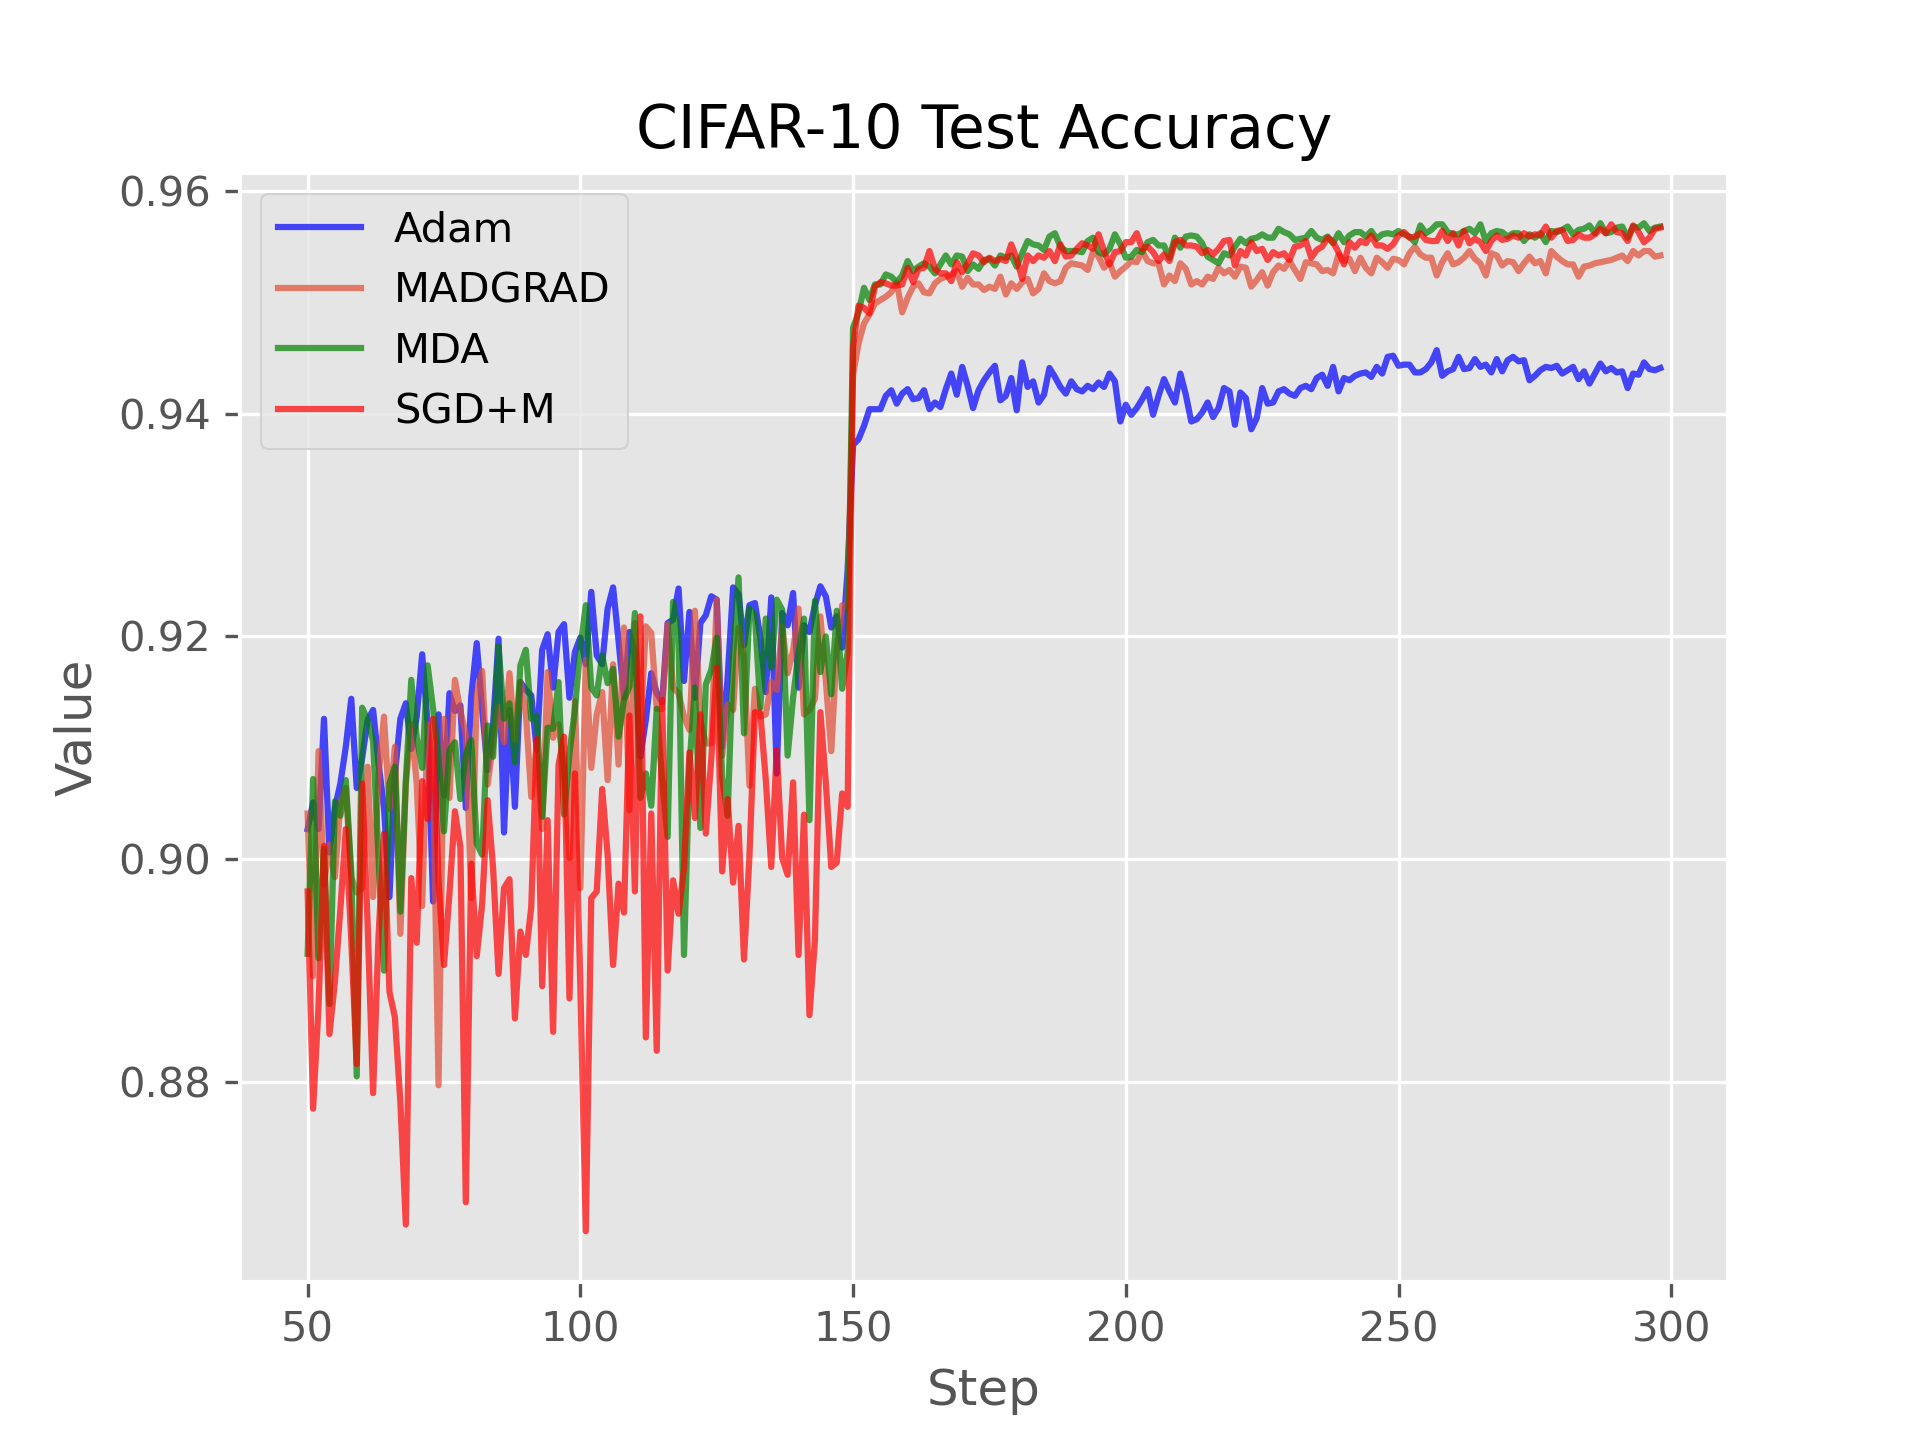
\includegraphics[width=\linewidth]{../ftrl_dl_data/CIFAR-10_test_acc_closeup.png}
    \caption{Test Accuracy of Optimizers on CIFAR-10}
    \label{fig:sub1}
  \end{subfigure}%
  \begin{subfigure}{.5\textwidth}
    \centering
    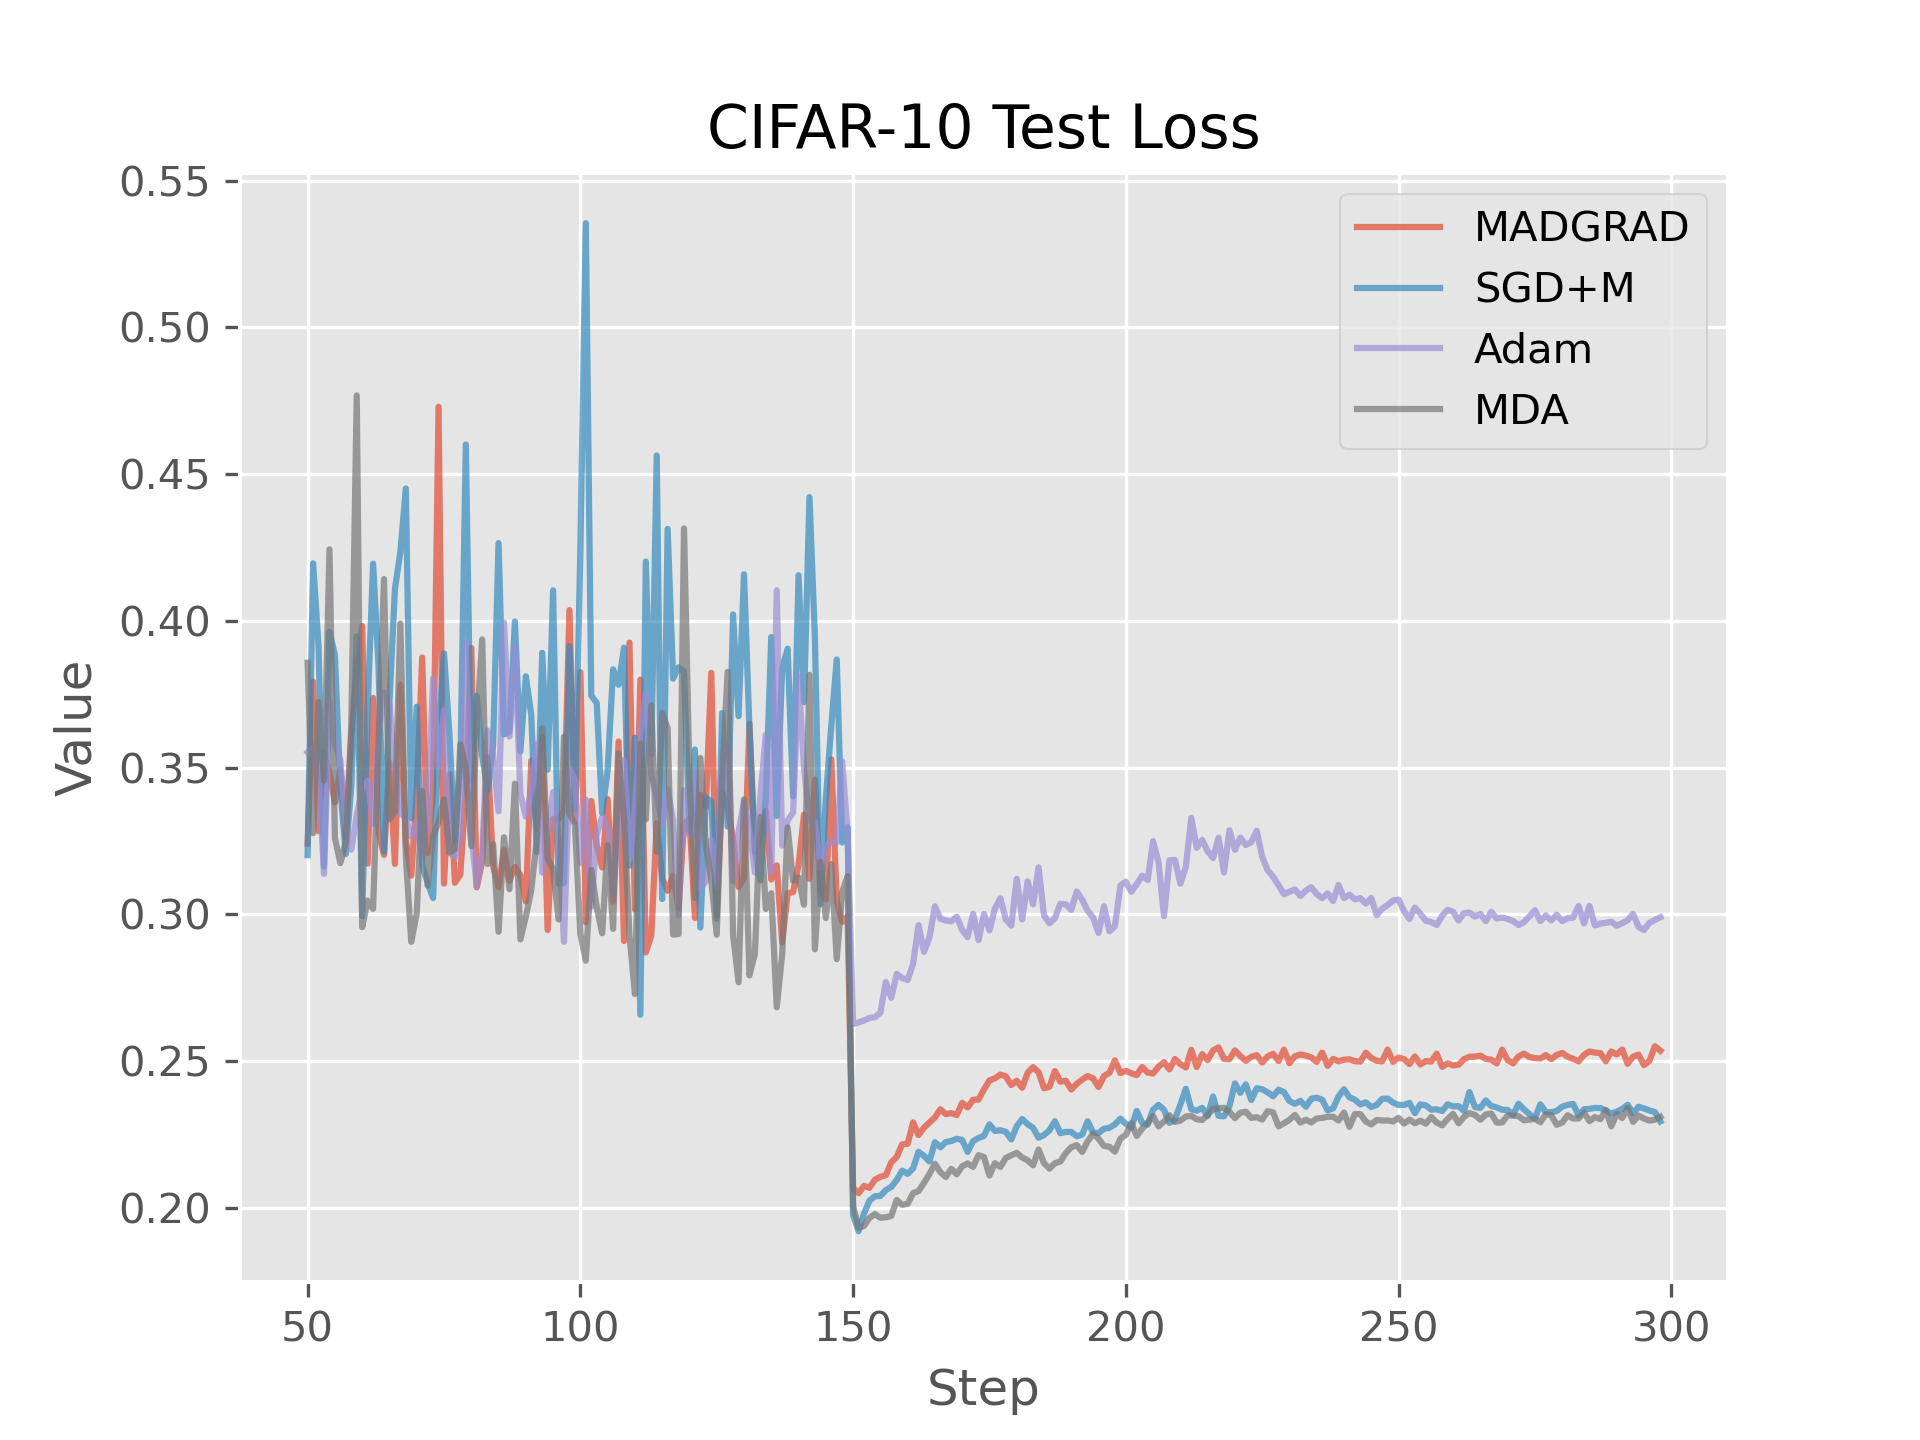
\includegraphics[width=\linewidth]{../ftrl_dl_data/CIFAR-10_test_loss_closeup.png}
    \caption{Test Loss of Optimizers on CIFAR-10}
    \label{fig:sub2}
  \end{subfigure}
  \caption{Comparison of optimizer performance on CIFAR-10 dataset}
  \label{fig:test}
\end{figure}
\end{frame}

\begin{frame}[shrink=15]
  \frametitle{MADGRAD Theory}
    \begin{itemize}
      \item In the original MADGRAD algorithm presented in the paper, the $z_{k+1}$ is given by:

      \[
        z_{k+1} = x_0 - \frac{1}{\sqrt[3]{v_{k+1}} + \epsilon} \circ s_{k+1}
      \]

      \item In the convergence proof, the $z_{k+1}$ parameter is given by:

      \[
        z_{k+1} = x_0 - \frac{1}{\sqrt[3]{\lambda_{k+1}G^2 + v_{k+1}}} \circ s_{k+1}
      \]

      \item This extra $\lambda_{k+1} G^2$ prevents the algorithm from being \emph{scale-free}, or an algorithm that is
        invariant to the scaling of losses by a constant factor
      \item Therefore, we aim to construct a convergence proof which maintains the scale-free nature of the algorithm,
        and does not require assumptions about the boundedness of the subgradients
      \item In particular, we avoid the asumption that $\|g_i\|_{\infty} \leq G$
      \item We make two reductions in order to prove our bound: we assume that $c_k = 1$ to only use FTRL updates, and
        we assume a constant learning rate
    \end{itemize}
\end{frame}

\begin{frame}
  \frametitle{Original MADGRAD Per-Coordinate Convergence Bound}
  \begin{align*}
    \E[f(x_k) 
    &- f(x_*)] \leq \frac{3}{\gamma}\frac{1}{(k+1)^{3/2}}\sum\limits_{d=0}^D\left(\E\left[\lambda_k
    \left(\sum\limits_{i=0}^k \lambda_i g_{i,d}^2\right)^{2/3}\right]\right) \\
    &+\frac{3}{\gamma}\frac{1}{(k+1)^{3/2}}\sum\limits_{d=0}^D(x_{0,d} - x_{*,d})^2\E\left(\lambda_{k+1}G^2 +
    \sum\limits_{i=1}^k\lambda_i g_{i,d}^2\right)^{1/3}
  \end{align*}
\end{frame}

\begin{frame}
  \frametitle{Lemma 1}
  \begin{restatable}[Lemma 1 in (Orabona and P\`al, 2015)~\cite{orabona_generalized_2014}]{lemma}{lemma1}\label{lemma:1}
    Let $\{\psi_t\}_{t=1}^\infty$ be a sequence of lower semi-continuous functions defined on a common convex domain $S
    \subseteq \R^n$ and such that each $\psi_t$ is $\mu_t$-strongly convex with respect to the norm $\|\cdot\|_t$. Let
    $\|\cdot\|_{t, *}$ be the dual norm of $\| \cdot \|_t$, for $t = 1, 2, \cdots, T$. Then, for any $\bu \in S$, the
    FTRL algorithm yields:

    \begin{align*}
      \Regret _T (\bu) \leq \sum\limits_{t=1}^T \langle g_t, \bu - \bx_t \rangle \leq \psi_{T}(\bu) + \psi_{1}^* (0) \\
      + \sum\limits_{t=1}^T B_{\psi_{t}^*}(-\theta_t, -\theta_{t-1}) - \psi_{t}^* (-\theta_t) + \psi_{t+1}^*(-\theta_t)
    \end{align*}
  \end{restatable}
\end{frame}

\begin{frame}
  \frametitle{Lemma 2}
  \begin{restatable}{lemma}{firstbound}\label{lemma:2}
    Let $a_1, a_2, \cdots, a_t$ be non-negative real numbers. If $a_1 > 0$, then
    \[
      \sum\limits_{t=1}^T \frac{a_t}{\sqrt[3]{\sum\limits_{s=1}^t a_s}} \leq \frac{3}{2}\left(\sum\limits_{t=1}^T
      a_t\right)^\frac{2}{3}
    \]
  \end{restatable}
\end{frame}

\begin{frame}
  \frametitle{Lemma 3}
  \begin{restatable}{lemma}{secondbound}\label{lemma:3}
    Let $C, a_1, a_2, \cdots, a_T \geq 0$, and $\alpha \geq 1, \alpha \neq \min\limits_{t=1,2,\cdots,T}a_{t}^\frac{4}{3}$.
    Then,

    \begin{align*}
      \sum\limits_{t=1}^T \min \left\{ \frac{a_{t}^2}{\sqrt[3]{\sum\limits_{s=1}^{t-1} a_{s}^2}}, C a_t\right\} \leq
      \frac{C \alpha}{\alpha - \min\limits_{t=1,2,\cdots,T}a_{t}^\frac{4}{3}} \max\limits_{t=1,2,\cdots,T} a_t
      + \\ 2\sqrt[3]{1 + \alpha^2} \sqrt{\sum\limits_{s=1}^T a_{s}^3}
    \end{align*}
  \end{restatable}
\end{frame}

\begin{frame}[shrink=20]
  \frametitle{Alternative MADGRAD Bound}
  \begin{restatable}{theorem}{regretbound}\label{theorem:1}
    Suppose $K \subseteq \R^D$ is a non-empty closed convex subset. Suppose that a regularizer $\psi_t: K \rightarrow \R$
    is a non-negative lower semi-continuous function that is strongly convex with respect to a norm $\| \cdot
    \|_{A_t}$. The regret of non-momentumized MADGRAD satisfies:

    \begin{align*}
      \Regret_T(\bu) \leq \sum\limits_{d=1}^D \frac{(\bu_d - x_{0,d})^2}{2\sqrt[3]{\sum\limits_{i=1}^{T} \lambda_i
        g_{i,d}^2}} &+ \frac{3}{2}\left(\sum\limits_{i=1}^T \lambda_i g_{i,d}^2\right)^\frac{2}{3} \\ +& 2
          \sqrt{T-1}\left(\sum_{i=1}^{T-1} \lambda_i g_{i,d}^2\right)^\frac{2}{3}(1 + \min_{t \leq
          T}(\sqrt{\lambda_t}|g_{t,d}|)^\frac{4}{3}) \max_{t \leq T} \sqrt{\lambda_t}|g_{td}| \\ &+ 2\sqrt[3]{1 + (1 +
          \min_{t \leq T}(\sqrt{\lambda_t}|g_{t,d}|)^\frac{4}{3})^2}\sqrt{\sum\limits_{t-1}^T \lambda_t^\frac{3}{2}
        |g_{t,d}|^3}
    \end{align*}
  \end{restatable}
\end{frame}

\begin{frame}[shrink=20]
  \frametitle{Proof Intuition}
  \begin{itemize}
    \item Our proof technique follows (Orabona and P\`al, 2015) for Scale-free Online Linear Opimization FTRL (SOLO FTRL)
    \item Our regularizer, $\psi_t(x) = \frac{1}{2}\|\bx - \bx_0\|_{A_t}$, is defined by a diagonal matrix, $A_t =
      \diag\left(\sqrt[3]{\sum\limits_{i=1}^{t-1} \lambda_i g_{i}^2}\right)$
    \item $\psi_t(\bx)$ is $\min_{d \leq D} \sqrt[3]{\sum\limits_{i=1}^{t-1} \lambda_i g_{i,d}^2}$-strongly convex
    \item Let $\eta_{t,d} = \frac{1}{\sqrt[3]{\sum_{i=1}^{t-1}}\lambda_i g_{i,d}^2}$
    \item We tighten this bound by analyzing in a per-parameter fashion by defining our regularizer in a per-coordinate
      manner: $\psi_{t,d}(x) = \frac{1}{\eta_{t,d}} \psi_{d}(\bx) = \frac{1}{2\eta_{t,d}}(\bx_d - \bx_{0,d})^2$
    \item Since $\psi_d(\bx): \R \rightarrow \R$, we can find the strong convexity constant by finding the lower bound
      of the second derivative of $\psi_d(\bx)$, which is 1.
    \item We use this per-coordinate regularizer in order to prove an entirely per-coordinate bound
  \end{itemize}
\end{frame}

\begin{frame}[shrink=20]
  \frametitle{Proof Technique}
  \begin{itemize}
    \item We start with Lemma 1, and upper bound the $B_{\psi_{t}^*}(-\theta_t, -\theta_{t-1}) - \psi_{t}^* (-\theta_t)
      + \psi_{t+1}^*(-\theta_t) \leq B_{\psi_{t}^*}(-\theta_t, -\theta_{t-1})$ in two ways using the properties of
      Fenchel conjugates, with the upper bound being the minimum of these two terms. Note that $H =
      \left(\sum\limits_{i=1}^{t-1} \lambda_i g_{i,d}^2\right)^\frac{2}{3} \sqrt{t-1}$

      \begin{align*}
        \Regret_T(\bu) &\leq \sum\limits_{d=1}^D \frac{1}{\eta_{T+1}}\psi_{d}(\bu) \frac{1}{\eta_1}\psi_{d}^*(0) \\
                       & + \sum\limits_{t=1}^T \min \left\{\frac{\eta_t \lambda_t g_{t,d}^2}{2}, \frac{\eta_{t+1,d}
                       \lambda_t g_{t,d}^2}{2} + H \sqrt{\lambda_t}|g_{t,d}|\right\} \\
        \therefore \Regret_T(\bu) &\leq \frac{1}{\eta_{T+1}}\psi_{d}(\bu) + \frac{1}{\eta_1}\psi_{d}^*(0) \\
                                  & +\frac{1}{2}\sum\limits_{t=1}^T \eta_{t+1} \lambda_t g_{t,d}^2 +
                                  \frac{1}{2}\sum\limits_{t=1}^T \min \left\{\frac{\eta_t \lambda_t g_{t,d}^2}{2},  2H
                                  \sqrt{\lambda_t}|g_{t,d}|\right\}
      \end{align*}

    \item We then use Lemma 3 to upper bound the minimum
    \item Lastly, we use Lemma 2 to upper bound the $\frac{1}{2}\sum\limits_{t=1}^T \eta_{t+1} \lambda_t g_{t,d}^2$
  \end{itemize}
\end{frame}

\begin{frame}
  \frametitle{Conclusion}
  \begin{itemize}
    \item In this work, we implement and analyze the performand of MDA and MADGRAD algorithms on the CIFAR10 dataset
    \item We then prove an alternate, scale-free regret bound for the MADGRAD algorithm
  \end{itemize}
\end{frame}

\begin{frame}[shrink=20]
  \frametitle{References}
  \bibliographystyle{ieeetr}
  \bibliography{../report/project_report}

  Code for PyTorch implementation, LaTeX for presentation and paper can be found at
  \href{https://github.com/shashankmanjunath/ftrl_deep_learning}{on GitHub at
  https://github.com/shashankmanjunath/ftrl\_deep\_learning}
\end{frame}
\end{document}
